\chapter{Variational Inference}\label{ch:vi}

The central computation in a probabilistic model is the posterior distribution of the unobserved variables given the observed ones. Exact inference (\cref{ch:inference}) is feasible only when the graph is a tree or has small cliques after elimination, and Markov chain Monte Carlo (\cref{ch:mcmc}) is asymptotically exact but slow and hard to diagnose. Variational inference takes a third route: it gives up exactness from the start and turns inference into \emph{optimization}. We choose a family of tractable distributions and search it for the member closest to the posterior. \Cref{sec:vi-posterior} states the problem, \cref{sec:kl} introduces the Kullback--Leibler divergence and the two ways of using it, and \cref{sec:mean-field} derives the classical mean-field algorithm for Markov random fields. \Cref{sec:elbo} rewrites the objective as the evidence lower bound, which only requires the unnormalized joint density, and \cref{sec:reparam} shows how to maximize it by stochastic gradients with the reparameterization trick. \Cref{sec:vi-vs-mcmc} compares the result with MCMC.

\section{Posterior Inference in Latent Variable Models}\label{sec:vi-posterior}

A \emph{latent variable model} specifies a joint distribution
\[
p(x,z)=p(z)\,p(x\given z),
\]
where $x$ are the observations, $z$ are the unobserved (latent) variables, $p(z)$ is the \emph{prior}, and $p(x\given z)$ is the \emph{likelihood}, the part of the model that gives the latent variables their meaning. Everything we want to know about $z$ after seeing $x$ is contained in the posterior
\[
p(z\given x)=\frac{p(x\given z)\,p(z)}{p(x)},\qquad p(x)=\int p(x,z)\dd z .
\]
The normalizing constant $p(x)$ is called the \emph{evidence} or \emph{marginal likelihood}.

\begin{remark}[TrueSkill]\label{rem:vi-trueskill}
The running example of the course is TrueSkill, a rating system for competitive games (\cref{ch:mcmc}). Each player $i$ has an unobserved skill $z_i$ with an independent Gaussian prior, and the probability that $i$ beats $j$ is $\sigma(z_i-z_j)$ with the logistic function $\sigma(t)=1/(1+e^{-t})$. With two players and a broad prior, the posterior after a few games is no longer Gaussian. After $A$ beats $B$ ten times it is confident that $z_A>z_B$; after each beats the other ten times it is confident that $z_A\approx z_B$ but remains uncertain about their common level. With $N$ players the posterior is a non-Gaussian density on $\R^N$, and the skills become dependent even for players who never met.
\end{remark}

When $z$ is high-dimensional the integral defining $p(x)$ is intractable, and with it most posterior computations:
\begin{enumerate}[(i)]
  \item the posterior density $p(z\given x)=p(z)p(x\given z)/p(x)$ itself;
  \item the evidence $p(x)$, used to compare models and to fit model parameters;
  \item marginals such as $p(z_1\given x)=\int p(z_1,\dots,z_D\given x)\dd z_2\cdots\dd z_D$, for example the skill of one player given all games;
  \item exact samples $z\sim p(z\given x)$, used to summarize plausible hypotheses, to predict, and to decide.
\end{enumerate}
What remains easy is the evaluation of the joint density $p(x,z)$ at a given pair $(x,z)$: the posterior is known up to its normalizing constant. Sampling methods exploit exactly this fact, and so does variational inference.

\begin{definition}[Variational Inference]\label{def:vi}
Given a target distribution $p(z\given x)$ and a family $\cQ$ of tractable distributions on the latent space, \emph{variational inference} computes
\[
q^*=\argmin_{q\in\cQ}\ \KL\big(q\,\|\,p(\cdot\given x)\big)
\]
by an iterative optimization method, and uses $q^*$ in place of the posterior. Typically $\cQ=\{q_\phi:\phi\in\Phi\}$ is parametric, for example $q_\phi=\cN(\mu,\Sigma)$ with $\phi=(\mu,\Sigma)$, or factorized, $q(z)=\prod_jq_j(z_j)$.
\end{definition}

Three choices define a variational method: the family $\cQ$, the measure of discrepancy, and the optimizer. Usually no member of $\cQ$ equals the posterior; the approximation error is the price paid for tractability.

\section{The Kullback--Leibler Divergence}\label{sec:kl}

\begin{definition}[KL Divergence]\label{def:kl}
For densities (or mass functions) $q$ and $p$ on the same space,
\[
\KL(q\,\|\,p)=\int q(z)\log\frac{q(z)}{p(z)}\dd z=\E_{z\sim q}\Big[\log\frac{q(z)}{p(z)}\Big],
\]
with the integral replaced by a sum in the discrete case.
\end{definition}

\begin{proposition}[Properties of the KL Divergence]\label{prop:kl-properties}
$\KL(q\,\|\,p)\ge0$, with equality if and only if $q=p$. In general $\KL(q\,\|\,p)\ne\KL(p\,\|\,q)$, so the KL divergence is not a metric.
\end{proposition}

Nonnegativity follows from Jensen's inequality applied to the concave logarithm. Asymmetry means there are two different ways to fit $q$ to $p$, and they behave very differently.

\begin{definition}[I-Projection and M-Projection]\label{def:projections}
Let $\cQ$ be a family of distributions and $p$ a target. The \emph{information projection} (I-projection) and the \emph{moment projection} (M-projection) of $p$ onto $\cQ$ are
\begin{align*}
q_I&=\argmin_{q\in\cQ}\KL(q\,\|\,p)=\argmin_{q\in\cQ}\E_{x\sim q}\Big[\log\frac{q(x)}{p(x)}\Big],\\
q_M&=\argmin_{q\in\cQ}\KL(p\,\|\,q)=\argmin_{q\in\cQ}\E_{x\sim p}\Big[\log\frac{p(x)}{q(x)}\Big].
\end{align*}
\end{definition}

The I-projection averages $\log(q/p)$ under $q$. It is large where $q$ puts mass and $p$ has almost none, so $q_I$ avoids such regions: it is \emph{mode seeking}, tends to lock onto one mode of a multimodal target, and underestimates the spread of $p$. The M-projection averages $\log(p/q)$ under $p$. It is large where $p$ has mass and $q$ has almost none, so $q_M$ must cover all of $p$: it is \emph{mass covering} and may put mass between the modes. \Cref{fig:projections} shows both for a bimodal target and the family of Gaussians.

\begin{figure}[ht]
\centering
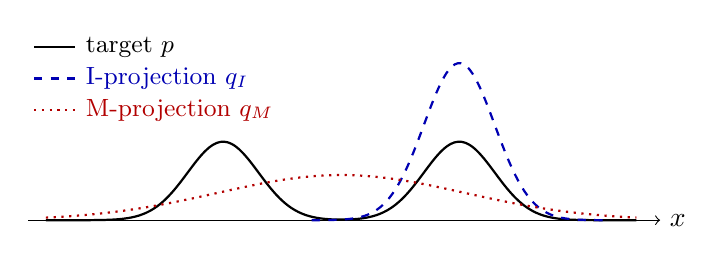
\begin{tikzpicture}[xscale=0.75,yscale=1]
  \draw[->] (-5.3,0) -- (5.4,0) node[right] {$x$};
  \draw[thick,domain=-5:5,samples=160,smooth] plot (\x,{3*(0.5*exp(-0.5*((\x+2)/0.6)*((\x+2)/0.6))+0.5*exp(-0.5*((\x-2)/0.6)*((\x-2)/0.6)))/(0.6*2.5066)});
  \draw[thick,dashed,blue!70!black,domain=-0.5:4.5,samples=100,smooth] plot (\x,{3*exp(-0.5*((\x-2)/0.6)*((\x-2)/0.6))/(0.6*2.5066)});
  \draw[thick,dotted,red!70!black,domain=-5:5,samples=120,smooth] plot (\x,{3*exp(-0.5*(\x/2.088)*(\x/2.088))/(2.088*2.5066)});
  \draw[thick] (-5.2,2.2) -- (-4.5,2.2) node[right,font=\small] {target $p$};
  \draw[thick,dashed,blue!70!black] (-5.2,1.8) -- (-4.5,1.8) node[right,font=\small] {I-projection $q_I$};
  \draw[thick,dotted,red!70!black] (-5.2,1.4) -- (-4.5,1.4) node[right,font=\small] {M-projection $q_M$};
\end{tikzpicture}
\caption{I- and M-projection of a bimodal density onto the Gaussian family. The I-projection fits one mode (the other mode gives an equally good, symmetric solution); the M-projection matches the mean and variance of $p$ and puts mass where $p$ has little.}
\label{fig:projections}
\end{figure}

\begin{proposition}[M-Projection onto an Exponential Family]\label{prop:m-projection}
Let $\cQ=\{q_\eta(x)=h(x)\exp(\eta\T T(x)-A(\eta))\}$ be an exponential family (\cref{sec:expfam}). If the M-projection $q_M=q_{\eta^*}$ exists, it matches the expected sufficient statistics of the target:
\[
\E_{x\sim q_{\eta^*}}[T(x)]=\E_{x\sim p}[T(x)].
\]
In particular, the M-projection onto the Gaussians has the mean and covariance of $p$.
\end{proposition}

Setting the gradient of $\KL(p\,\|\,q_\eta)=\text{const}-\eta\T\E_p[T(x)]+A(\eta)$ to zero gives $\nabla A(\eta)=\E_p[T(x)]$, and $\nabla A(\eta)=\E_{q_\eta}[T(x)]$ is the mean of the sufficient statistics.

\begin{remark}[Connection to Maximum Likelihood]\label{rem:mle-m-projection}
If $p$ is the empirical distribution of a sample $x_1,\dots,x_n$, then $\KL(p\,\|\,q_\theta)=\text{const}-\frac1n\sum_{i}\log q_\theta(x_i)$. Maximum likelihood estimation (\cref{sec:mle}) is therefore the M-projection of the data onto the model, and \cref{prop:m-projection} is the moment-matching property of exponential-family MLEs from \cref{sec:expfam}.
\end{remark}

\begin{remark}[Maximum Entropy]
The entropy $\cH(p)=-\E_{x\sim p}[\log p(x)]$ measures the uncertainty of $p$. Among all distributions satisfying the moment constraints $\E_p[f_i(x)]=t_i$, $i=1,\dots,k$, the entropy is maximized by an exponential family with sufficient statistics $(f_1,\dots,f_k)$. Exponential families are therefore the least committal distributions consistent with given moments, which is another reason they are the natural variational families.
\end{remark}

Which direction should we use for inference? The M-projection is attractive, since it gets the moments right, but it requires expectations under $p(z\given x)$, which is exactly what we cannot compute. The I-projection only requires expectations under $q$, which we choose to be tractable. Almost all variational inference algorithms therefore use the I-projection, $\KL(q\,\|\,p)$, and inherit its mode-seeking behavior.

\section{Mean-Field Approximation}\label{sec:mean-field}

We first apply the I-projection to a Markov random field (\cref{sec:mrf}). In this section $x=(x_1,\dots,x_N)$ denotes all variables of the field (any observed variables have already been fixed, as in the denoising example of \cref{sec:loopy-bp}), and
\[
p(x)=\frac1Z\prod_{C\in\cC}\psi_C(x_C)=\exp\Big(\sum_{C\in\cC}\log\psi_C(x_C)-\log Z\Big).
\]
For any $q$,
\[
\KL(q\,\|\,p)=\E_q[\log q(x)]-\sum_{C\in\cC}\E_q[\log\psi_C(x_C)]+\log Z,
\]
and since $\log Z$ does not depend on $q$,
\begin{equation}\label{eq:vi-mrf-objective}
q^*=\argmin_{q\in\cQ}\KL(q\,\|\,p)=\argmax_{q\in\cQ}\Big\{\sum_{C\in\cC}\E_q[\log\psi_C(x_C)]+\cH(q)\Big\}.
\end{equation}
The intractable partition function has dropped out. The objective trades off fitting the potentials, which favors concentrating $q$ on high-potential configurations, against the entropy, which keeps $q$ spread out. If $p\in\cQ$ the solution is $q^*=p$, but this almost never happens for a tractable $\cQ$.

\begin{definition}[Naive Mean-Field Family]\label{def:mean-field}
The \emph{(naive) mean-field family} consists of the fully factorized distributions $q(x)=\prod_{i=1}^Nq_i(x_i)$.
\end{definition}

Under this family both terms of \eqref{eq:vi-mrf-objective} simplify. The marginal of a clique is a product, $q(x_C)=\prod_{i\in C}q_i(x_i)$, and the entropy is additive, $\cH(q)=\sum_i\cH(q_i)$, because $\log q(x)=\sum_i\log q_i(x_i)$ and each term only involves one coordinate. For a pairwise MRF with edge set $E$ and potentials $\psi_{ij}$ the problem becomes
\begin{equation}\label{eq:vi-pairwise}
\max_{q_1,\dots,q_N}\ \sum_{(i,j)\in E}\sum_{x_i,x_j}q_i(x_i)\,q_j(x_j)\log\psi_{ij}(x_i,x_j)-\sum_{i}\sum_{x_i}q_i(x_i)\log q_i(x_i)
\end{equation}
subject to $q_i(x_i)\ge0$ and $\sum_{x_i}q_i(x_i)=1$. This objective is not concave jointly and has many local maxima, but it is easy to maximize over one factor $q_i$ with the others fixed. Writing the Lagrangian for the normalization constraint, differentiating with respect to $q_i(x_i)$, and setting the derivative to zero gives the closed-form update
\begin{equation}\label{eq:mf-update}
q_i(x_i)\propto\exp\Big(\sum_{j\in N(i)}\sum_{x_j}q_j(x_j)\log\psi_{ij}(x_i,x_j)\Big),
\end{equation}
where $N(i)$ is the set of neighbors of $i$. If the field also has node potentials $\psi_i(x_i)$, the term $\log\psi_i(x_i)$ is added inside the exponential.

\begin{algorithm}[H]
\caption{Naive Mean-Field (Coordinate Ascent)}\label{alg:mean-field}
\begin{algorithmic}[1]
\Input{Pairwise MRF with potentials $\psi_{ij}$ on the edges $E$ (and optionally node potentials $\psi_i$); tolerance $\epsilon$.}
\Init{$q_i$ uniform on the states of $x_i$, for every node $i$.}
\Repeat
  \For{$i=1,\dots,N$} \Comment{any fixed or random order}
    \State $\ell_i(x_i)\gets\log\psi_i(x_i)+\sum_{j\in N(i)}\sum_{x_j}q_j(x_j)\log\psi_{ij}(x_i,x_j)$ for every state $x_i$
    \State $q_i(x_i)\gets\exp(\ell_i(x_i))\big/\sum_{x'}\exp(\ell_i(x'))$
  \EndFor
\Until{the objective \eqref{eq:vi-pairwise}, plus the node terms $\sum_i\sum_{x_i}q_i(x_i)\log\psi_i(x_i)$, increases by less than $\epsilon$}
\Output{Factors $q_1,\dots,q_N$; $q_i$ approximates the marginal $p(x_i)$.}
\end{algorithmic}
\end{algorithm}

Each update maximizes the objective exactly in one block of variables, so the objective never decreases and the algorithm converges, but only to a local maximum that depends on the initialization and the update order. The output approximates each marginal by $q_i$ and ignores all correlations between variables.

\begin{remark}[Mean Field for the Ising Model]\label{rem:mf-ising}
For the Ising model (\cref{sec:ising}) with spins $x_i\in\{-1,+1\}$ and $p(x)\propto\exp\big(\sum_ib_ix_i+\sum_{(i,j)\in E}J_{ij}x_ix_j\big)$, the update \eqref{eq:mf-update} gives $q_i(x_i)\propto\exp\big(x_i(b_i+\sum_{j\in N(i)}J_{ij}\mu_j)\big)$, where $\mu_j=\E_{q_j}[x_j]$. In terms of the means,
\[
\mu_i\gets\tanh\Big(b_i+\sum_{j\in N(i)}J_{ij}\mu_j\Big).
\]
Each spin feels the \emph{average} field produced by its neighbors, which is the origin of the name ``mean field''. Applied to the noisy-image MRF of \cref{sec:loopy-bp}, the rounded means $\sign(\mu_i)$ give a denoised image.
\end{remark}

\begin{remark}[Connection to Gibbs Sampling and Belief Propagation]\label{rem:mf-gibbs}
The Gibbs sampler (\cref{alg:gibbs}) visits the nodes in turn and draws $x_i$ from $p(x_i\given x_{N(i)})\propto\exp\big(\sum_{j\in N(i)}\log\psi_{ij}(x_i,x_j)\big)$, using the current \emph{values} of the neighbors. Mean field performs the same sweep but replaces the neighbors' values by \emph{averages} under $q_j$; it is a deterministic, averaged version of Gibbs sampling. Loopy belief propagation (\cref{alg:loopy-bp}) is another local, iterative scheme on the same graph; it sends edge-specific messages instead of one shared belief per node, and its fixed points correspond to a different variational objective.
\end{remark}

\section{The Evidence Lower Bound}\label{sec:elbo}

We return to a general latent variable model $p(x,z)$ and a parametric family $q_\phi(z)$. The objective $\KL(q_\phi\,\|\,p(\cdot\given x))$ cannot be evaluated, because it involves the normalized posterior. Expanding $p(z\given x)=p(x,z)/p(x)$ separates the unknown constant:
\begin{align*}
\KL\big(q_\phi(z)\,\|\,p(z\given x)\big)
&=\E_{z\sim q_\phi}\Big[\log\frac{q_\phi(z)\,p(x)}{p(x,z)}\Big]
=-\E_{z\sim q_\phi}\big[\log p(x,z)-\log q_\phi(z)\big]+\log p(x).
\end{align*}

\begin{definition}[Evidence Lower Bound]\label{def:elbo}
The \emph{evidence lower bound} (ELBO) of $q_\phi$ is
\[
\ELBO(\phi)=\E_{z\sim q_\phi}\big[\log p(x,z)-\log q_\phi(z)\big]=\E_{z\sim q_\phi}[\log p(x,z)]+\cH(q_\phi).
\]
\end{definition}

\begin{theorem}[ELBO Identity]\label{thm:elbo}
For every $q_\phi$,
\[
\log p(x)=\ELBO(\phi)+\KL\big(q_\phi(z)\,\|\,p(z\given x)\big).
\]
Consequently $\ELBO(\phi)\le\log p(x)$, with equality if and only if $q_\phi=p(\cdot\given x)$, and maximizing the ELBO over $\phi$ is equivalent to minimizing the KL divergence to the posterior.
\end{theorem}

The theorem is the rearranged display above together with $\KL\ge0$. The left side does not depend on $\phi$, so every increase of the ELBO is a decrease of the KL divergence by the same amount. The ELBO only involves the joint density $p(x,z)$, which we can evaluate, and expectations under $q_\phi$, which we can sample. It has two readings:
\begin{itemize}
  \item \emph{expected log-joint plus entropy}: $\E_{q_\phi}[\log p(x,z)]$ pulls $q_\phi$ toward configurations that explain the data and agree with the prior, while $\cH(q_\phi)$ prevents it from collapsing onto a single point;
  \item \emph{expected log-likelihood minus KL to the prior}: since $\log p(x,z)=\log p(x\given z)+\log p(z)$,
  \begin{equation}\label{eq:elbo-recon-kl}
  \ELBO(\phi)=\E_{z\sim q_\phi}[\log p(x\given z)]-\KL\big(q_\phi(z)\,\|\,p(z)\big),
  \end{equation}
  which rewards explaining the data and penalizes moving away from the prior. This is the form used by variational autoencoders (\cref{sec:vae}).
\end{itemize}

\begin{remark}[Mean Field Revisited]
For an MRF the role of the evidence is played by the partition function: with the unnormalized density $\tilde p(x)=\prod_C\psi_C(x_C)$, the objective in \eqref{eq:vi-mrf-objective} is exactly $\E_q[\log\tilde p(x)]+\cH(q)$, and the same argument gives $\log Z=\text{objective}+\KL(q\,\|\,p)$. Mean field (\cref{alg:mean-field}) is coordinate ascent on an ELBO over a factorized family. The general version of the update, $q_j(z_j)\propto\exp\big(\E_{q_{-j}}[\log p(x,z)]\big)$, where the expectation is over all other factors, is known as coordinate ascent variational inference (CAVI).
\end{remark}

\begin{remark}[Connection to EM]
The ELBO is also a function of model parameters $\theta$ when the joint density is $p_\theta(x,z)$, and $\log p_\theta(x)\ge\ELBO(\theta,\phi)$ for every $\phi$. Alternating between maximizing over $q$ and over $\theta$ is the EM algorithm of \cref{sec:em}; maximizing over both by stochastic gradients is the variational autoencoder of \cref{sec:vae}.
\end{remark}

\section{Stochastic Gradients and the Reparameterization Trick}\label{sec:reparam}

Coordinate updates in closed form exist only for special models. For a general differentiable model we maximize the ELBO by gradient ascent, $\phi\gets\phi+\eta\,\nabla_\phi\ELBO(\phi)$, as in \cref{sec:gd}. The gradient is an expectation that we cannot compute exactly, so we use an unbiased Monte Carlo estimate (\cref{sec:mc-estimation}) and stochastic gradient ascent (\cref{sec:sgd}).

The difficulty is that the distribution over which we average depends on $\phi$. If $Y$ had a distribution not depending on $\phi$, we could exchange gradient and expectation, $\nabla_\phi\E[f(Y,\phi)]=\E[\nabla_\phi f(Y,\phi)]\approx\frac1m\sum_{k=1}^m\nabla_\phi f(y_k,\phi)$. For the ELBO, however,
\[
\nabla_\phi\E_{z\sim q_\phi}\big[\log p(x,z)-\log q_\phi(z)\big]\ne\E_{z\sim q_\phi}\big[\nabla_\phi\big(\log p(x,z)-\log q_\phi(z)\big)\big],
\]
because moving $\phi$ also moves the samples.

\begin{definition}[Reparameterization]\label{def:reparam}
A family $q_\phi$ is \emph{reparameterizable} if there are a fixed base distribution $p_0$, not depending on $\phi$, and a map $T$, differentiable in $\phi$, such that
\[
\varepsilon\sim p_0\quad\Longrightarrow\quad z=T(\varepsilon,\phi)\sim q_\phi .
\]
\end{definition}

The standard example is the Gaussian family: with $\phi=(\mu,\sigma)$, $\varepsilon\sim\cN(0,I)$, and $z=\mu+\sigma\odot\varepsilon$, we have $z\sim\cN(\mu,\diag(\sigma^2))$. The randomness now enters through $\varepsilon$, whose distribution is fixed, and $\phi$ enters only through a deterministic, differentiable map. Hence
\begin{equation}\label{eq:reparam-grad}
\begin{aligned}
\nabla_\phi\ELBO(\phi)&=\E_{\varepsilon\sim p_0}\Big[\nabla_\phi\big(\log p\big(x,T(\varepsilon,\phi)\big)-\log q_\phi\big(T(\varepsilon,\phi)\big)\big)\Big]\\
&\approx\frac1m\sum_{k=1}^m\nabla_\phi\big(\log p(x,z_k)-\log q_\phi(z_k)\big)\Big|_{z_k=T(\varepsilon_k,\phi)},
\end{aligned}
\end{equation}
where the gradient flows through $z_k=T(\varepsilon_k,\phi)$ by the chain rule. In code, one writes the Monte Carlo ELBO as a function of $\phi$ and lets automatic differentiation (\cref{sec:backprop}) do the rest.

\begin{algorithm}[H]
\caption{Stochastic Variational Inference with Reparameterization}\label{alg:svi}
\begin{algorithmic}[1]
\Input{Data $x$; joint density $p(x,z)$, differentiable in $z$; reparameterizable family $q_\phi$ with base distribution $p_0$ and map $T$; Monte Carlo sample size $m$; learning rates $\eta_t$; number of iterations $K$.}
\Init{Variational parameters $\phi$, e.g.\ $\mu=0$ and $\log\sigma=0$ for a Gaussian family.}
\For{$t=1,\dots,K$}
  \State Draw $\varepsilon_1,\dots,\varepsilon_m\iidsim p_0$ and set $z_k\gets T(\varepsilon_k,\phi)$.
  \State $\widehat{\ELBO}(\phi)\gets\frac1m\sum_{k=1}^m\big(\log p(x,z_k)-\log q_\phi(z_k)\big)$
  \State $\hat g\gets\nabla_\phi\widehat{\ELBO}(\phi)$ \Comment{differentiate through $z_k=T(\varepsilon_k,\phi)$}
  \State $\phi\gets\phi+\eta_t\,\hat g$ \Comment{gradient \emph{ascent}; in practice Adam}
\EndFor
\Output{Approximate posterior $q_\phi\approx p(z\given x)$.}
\end{algorithmic}
\end{algorithm}

The estimate $\hat g$ is unbiased for every $m\ge1$; larger $m$ reduces its variance at proportional cost, and $m=1$ is common. The method only needs to evaluate $\log p(x,z)$ and its gradient in $z$, so it applies to any model with continuous latent variables, such as TrueSkill with a Gaussian approximation to the skills. When the data consist of many conditionally independent points, $\log p(x,z)$ is a sum over data points and can be replaced by a rescaled minibatch sum, which is a second source of stochasticity in the same spirit as \cref{alg:sgd}.

\begin{remark}[Score-Function Estimator]
An alternative that does not require reparameterization uses the log-derivative trick $\nabla_\phi q_\phi=q_\phi\nabla_\phi\log q_\phi$:
\[
\nabla_\phi\E_{z\sim q_\phi}[f(z)]=\E_{z\sim q_\phi}\big[f(z)\,\nabla_\phi\log q_\phi(z)\big].
\]
It works for discrete latent variables and non-differentiable $f$, and it is the same identity that underlies the policy gradient theorem in reinforcement learning. Its variance is usually much larger than that of \eqref{eq:reparam-grad}, because it only uses the value of $f$, not its gradient.
\end{remark}

\section{Variational Inference versus MCMC}\label{sec:vi-vs-mcmc}

MCMC (\cref{ch:mcmc}) and variational inference answer the same question with opposite trade-offs.

\begin{center}
\small
\begin{tabularx}{\textwidth}{@{}l>{\raggedright\arraybackslash}X>{\raggedright\arraybackslash}X@{}}
\toprule
 & MCMC & Variational inference \\
\midrule
Output & samples whose distribution converges to $p(z\given x)$ & a distribution $q^*\in\cQ$ \\
Accuracy & asymptotically exact & biased by the choice of $\cQ$, even with infinite compute \\
Multimodality & can visit several modes (slowly) & I-projection is mode seeking \\
Cost & many iterations; samples are correlated & optimization; fast and scalable with SGD \\
Tuning & proposal scales, step sizes, burn-in; convergence is hard to diagnose (\cref{sec:mcmc-diagnostics}) & learning rate, family, initialization; convergence is monitored through the ELBO \\
Typical use & accurate posterior summaries for moderate models & large models and data sets; inner loop of learning (VAEs) \\
\bottomrule
\end{tabularx}
\end{center}

\begin{notebox}{Pros and Cons}
Variational inference replaces sampling by optimization, so it converges quickly, scales to large data sets through stochastic gradients, and is easy to implement with automatic differentiation; the ELBO provides a usable objective and a lower bound on the evidence. However, the result is only as good as the family $\cQ$: a factorized or Gaussian $q$ ignores correlations and non-Gaussian shape, the I-projection underestimates posterior uncertainty and picks a single mode, and the answer is sensitive to initialization and learning rates.
\end{notebox}

\begin{notebox}{Limitations and what comes next}
So far the model $p(x,z)$ was fixed and we approximated one posterior. In unsupervised learning the model has parameters $\theta$ of its own, to be fitted by maximizing the evidence $p_\theta(x)$, and every data point $x_i$ has its own latent variable $z_i$ and therefore its own posterior. \Cref{ch:latent} handles both. When the posterior is tractable, maximizing the ELBO alternately over $q$ and $\theta$ gives the EM algorithm; when it is not, a neural network that maps each $x_i$ to the parameters of $q(z_i\given x_i)$ amortizes the cost of inference, and training it jointly with $\theta$ by \cref{alg:svi} gives the variational autoencoder.
\end{notebox}
